\documentclass[a4paper,12pt]{article}
%\documentclass[doc]{apa}
\usepackage[usenames,dvipsnames]{color}
\usepackage{graphicx}
\usepackage{multicol}
\usepackage{multirow}
\usepackage{amsmath}
\usepackage{hyperref}
\usepackage{pdfpages}

%\setlength\parindent{0pt}
%\usepackage{figure}
\usepackage[margin=0.8in]{geometry}
\title{Project 2 - 3D Reconstruction from two views}
\author{Daniel Bryan and Olmo Zavala\\Florida State University}

\begin{document}
\maketitle

\section{Description}
The objective of this project is to implement the normalized eight-point algorithm 
for estimating the fundamental matrix, and how to generate 3D models from images. \\

\section{Eight-point algorithm}
Our implementation of the 8-pt algorithm is based on the slides of the class and it basically
follows the following algorithm:
\begin{itemize}
    \item Normalize image points
        \begin{itemize}
            \item \textbf{Centroid is at the origin}. We create the matrix $T_{trans}$ for each
                camera like this:
                \begin{equation}
                    \left [
                    \begin{array}[ ]{c c c}
                        1 & 0 & -\mu_x\\
                        0 & 1 & -\mu_y\\
                        0 & 0 & 1\\
                    \end{array}
                \right ]
                \end{equation}
                And we multiply each point of the cameras to they corresponding $T$ matrix like this:
                $Tx_i$.
            \item \textbf{RMS distance from the origin is $\sqrt{2}$.} First compute the RMS of the
                available points:
                \begin{equation}
                    \sqrt{ \frac{1}{n} \sum_{i=1}^n \left(  (x_i - \mu_x)^2 + (y_i- \mu_y)^2) \right) }
                \end{equation}
                Then create $T_{scale}$ and multiply it to each point in the camera. T is:
                \begin{equation}
                    T_s = \left[ 
                    \begin{array}[]{ccc}
                        \sqrt{2}/RMS & 0 & 0 \\
                        0 & \sqrt{2}/RMS  & 0 \\
                        0 & 0 & 1 
                    \end{array}
                     \right]
                \end{equation}
        \end{itemize}
    \item \textbf{Multiply each point by $T_n = T_sT_t$ like this $[u~ v~ 1]' = T_nx$. Do it for each camera.}
    \item \textbf{Solve $x'_nFx_n = 0$ }. To do this we need to form the system $Af = 0$ and solve for f.
        The matrix A is: \begin{equation}
            A = \left[ 
            \begin{array}[ ]{ccccccccc}
                u'_1u_1 & u'_1v_1 & u'_1 & v'_1u_1 &v'_1v_1 & v'_1 & u_1 & v_1 & 1 \\
                u'_2u_2 & u'_2v_2 & u'_2 & v'_2u_2 &v'_2v_2 & v'_2 & u_2 & v_2 & 1 \\
                u'_3u_3 & u'_3v_3 & u'_3 & v'_3u_3 &v'_3v_3 & v'_3 & u_3 & v_3 & 1 \\
                &&& \vdots \\
                u'_nu_n & u'_nv_n & u'_n & v'_nu_n &v'_nv_n & v'_n & u_n & v_n & 1 
            \end{array}
            \right] F = 0
        \end{equation}
    \item \textbf{Find least square solution of $Af = 0$}. 
        \begin{itemize}
            \item First find SVD of A ($USV^T = A$).
            \item Choose $F_{Norm}$ to be the last column of V
        \end{itemize}
    \item \textbf{Enforcing Singularity} 
        \begin{itemize}
            \item For $F_{Norm}=USV^T$ 
            \item Set $S_3$=0 for 
            \begin{equation}
                       F_{norm} =U \left[ 
            \begin{array}[]{ccc}
                        S_1 & 0 & 0 \\
                        0 & S_2  & 0 \\
                        0 & 0 & S_3 
                    \end{array}
            \right] V^T
            \end{equation}
        \end{itemize}
    \item \textbf{Denormalisation}
    	\begin{equation}
    	F=T_{NormLeft}*F_{Norm}*T_{NormRight}
    	\end{equation}
    \item \textbf{Compute essential matrix E}
        \begin{equation}
            E =  K^T*F*K 
        \end{equation}
        Where K are the intrinsic camera parameters of the Kinect camera:
            \begin{equation}
                       K = \left[ 
            \begin{array}[]{ccc}
                        -525 & 0 & 320 \\
                        0 & -525 & 240 \\
                        0 & 0 & 1 \\
                    \end{array}
            \right] 
            \end{equation}
        \item \textbf{Estimate R and T from E}
            \begin{itemize}
                \item SVD on E. $E = USV^T$
                \item $R  = UWV^T$ or $R = UW^TV^T$. Where W i given by 
                    \begin{equation}
                        W = \left [ 
                            \begin{array}[]{ccc}
                                0 & -1 & 0  \\
                                1 & 0 & 0   \\
                                0 & 0 & 1
                            \end{array}
                            \right ] 
                    \end{equation}
                \item T can be $u_3$ or $-u_3$.
            \end{itemize}
        \item {Choose proper solution}. Finally we need to choose from the four
            possible solutions the one twhere 
    \end{itemize}

    \section{Interface to define corresponding points.}
    We created a useful Matlab interface to define the corresponding points between two images.
    Figure \ref{fig:demo} shows a screen shot of this interface. The user needs to select
    corresponding points between images and it doesn't have to be in order (one point in one
    image and the next point in the following image). The interface also provides a button to
    reset all the points as well as to remove the last added point. These two buttons are
    very handy when selecting points. Once all the desired buttons have been selected the 
    resulting points are saved in at matlab file that can be stored for later compuatation
    using the 8-point algorithm. 

    \begin{figure}[h]
        \centering
        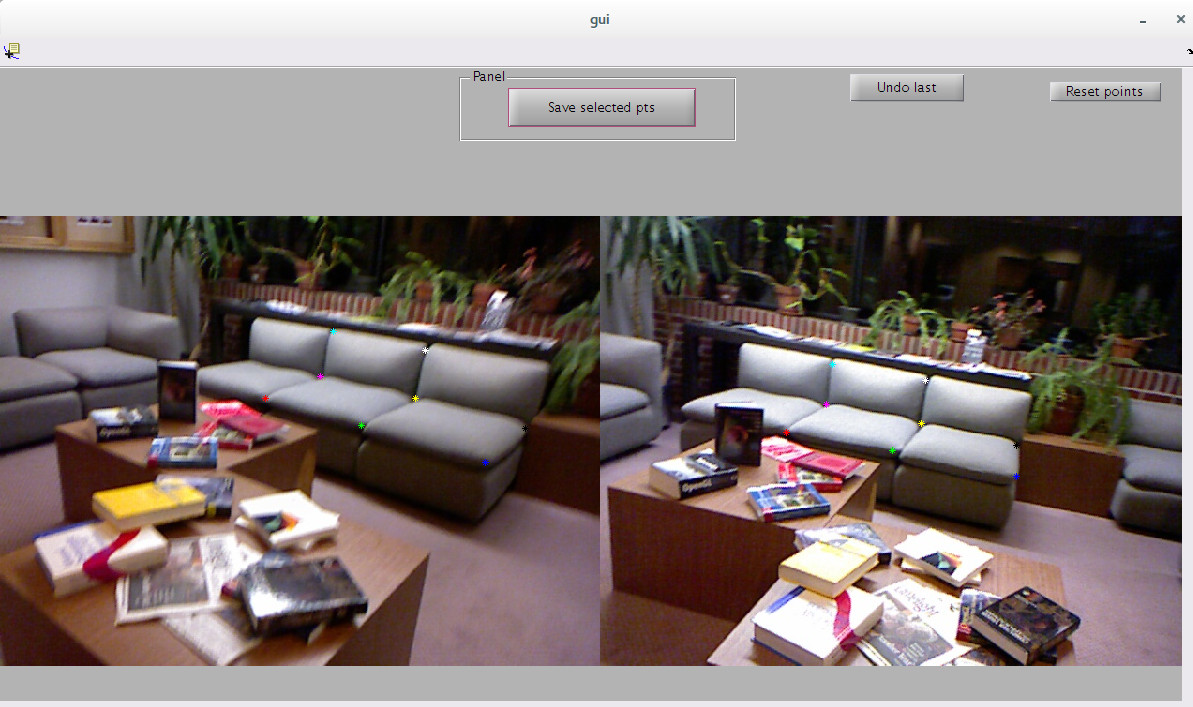
\includegraphics[totalheight=.38\textheight]{./images/Example.jpg}
        \caption{Matlab interface to select corresponding points between two images.
        Example of selecting 9 points using the Matlab interface.}
        \label{fig:demo}
    \end{figure}

    Each corresponding point is displayed with the same color, 
    this makes it easy to see wich points correspond in both of the images.
    The coordinates obtained from the selection of points displayed at figure \ref{fig:demo} 
    are displayed in figure \ref{fig:pts}.

    \begin{figure}[h]
        \centering
        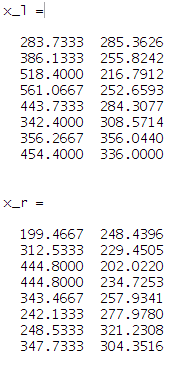
\includegraphics[totalheight=.24\textheight]{./images/ExamplePts.png}
        \caption{Obtained coordinates from the selected in figure \ref{fig:demo}.}
        \label{fig:pts}
    \end{figure}

    In our results we use the example provided by the professor to compare the results. \\

    In order to test the correct coordinates of the points obtained by the Matlab interface
    we selected 4-points close to the corners of the two figures as displayed in figure \ref{fig:check}. 
    The points start in the upper right corner and go clockwise until the upper left corner. 
    The values obtained correspond very closely with the dimensions of the images but with the
    origin in the lower left corner. The values obtained are also displayed in figure \ref{fig:check}.
    \begin{figure}[h]
        \centering
        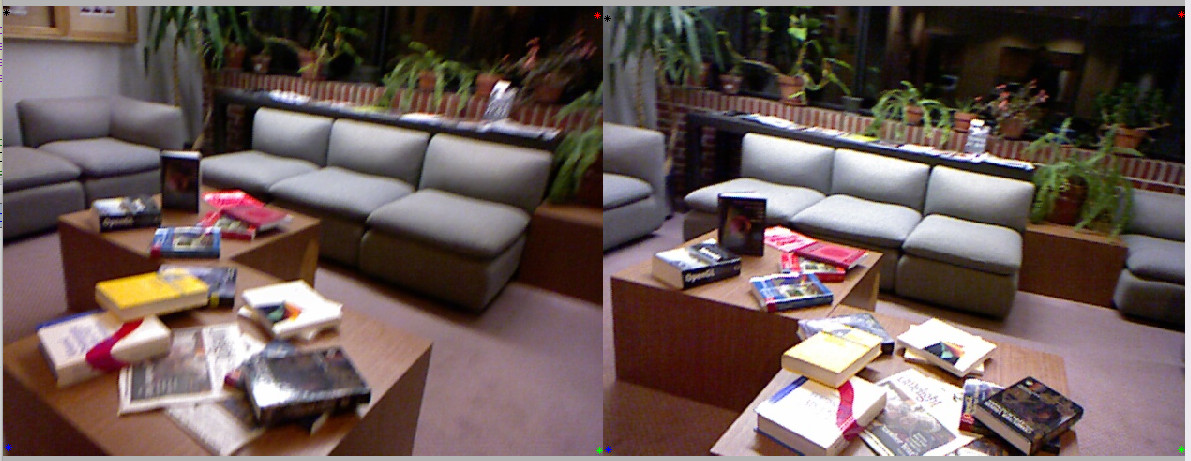
\includegraphics[totalheight=.20\textheight]{./images/Test.jpg}
        \vspace{1px}
        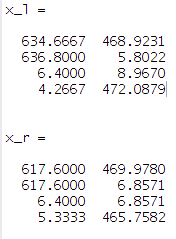
\includegraphics[totalheight=.18\textheight]{./images/TestPts.png}
        \caption{Corners used to test the proper coordinates of the Matlab interface.}
        \label{fig:check}
    \end{figure}

    \section{Results}
    To test our results we use the example provided by the profesor. This example were
    12 points with the coordinates shown in figure \ref{fig:epts}.
    \begin{figure}[h]
        \centering
        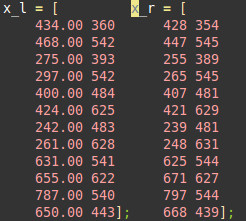
\includegraphics[totalheight=.20\textheight]{./images/Ppts.jpg}
        \caption{Coordinates used to test our results.}
        \label{fig:epts}
    \end{figure}


    \end{document}
